\begin{document}
\title{\Large \lecture \\ \textbf{\normalsize \assignment}}
\author{\authors}

\setlength \headheight{25pt}
\fancyhead[R]{\begin{tabular}{r}\lecture \\ \assignment \end{tabular}}
\fancyhead[L]{\authors}

\maketitle

\section{Introduction}
The goal of this project is to transfer textfiles as sequence of characters through a network with reliable data transfer. \ifthenelse{\boolean{m2}}{In this paper we will present our ideas for the layering of our protocol.}{In this paper we will present our final layering and protocol design.}

\section{Layering and Protocol Design}

Beside the two layers, physical and application layer, Cnet provides we implement three additional layers between them. We call them \emph{link layer}, \emph{network layer}, and \emph{transport layer}, from bottom to top. Data packets in the link layer are called \emph{frame}, in the network layer \emph{datagram} and in the transport layer \emph{segment}. To data packets from the application layer we refer to as \emph{messages}. Figure~\ref{fig:overview-layers} gives an overview how the different layers call each other.

\begin{figure}
  \centering
  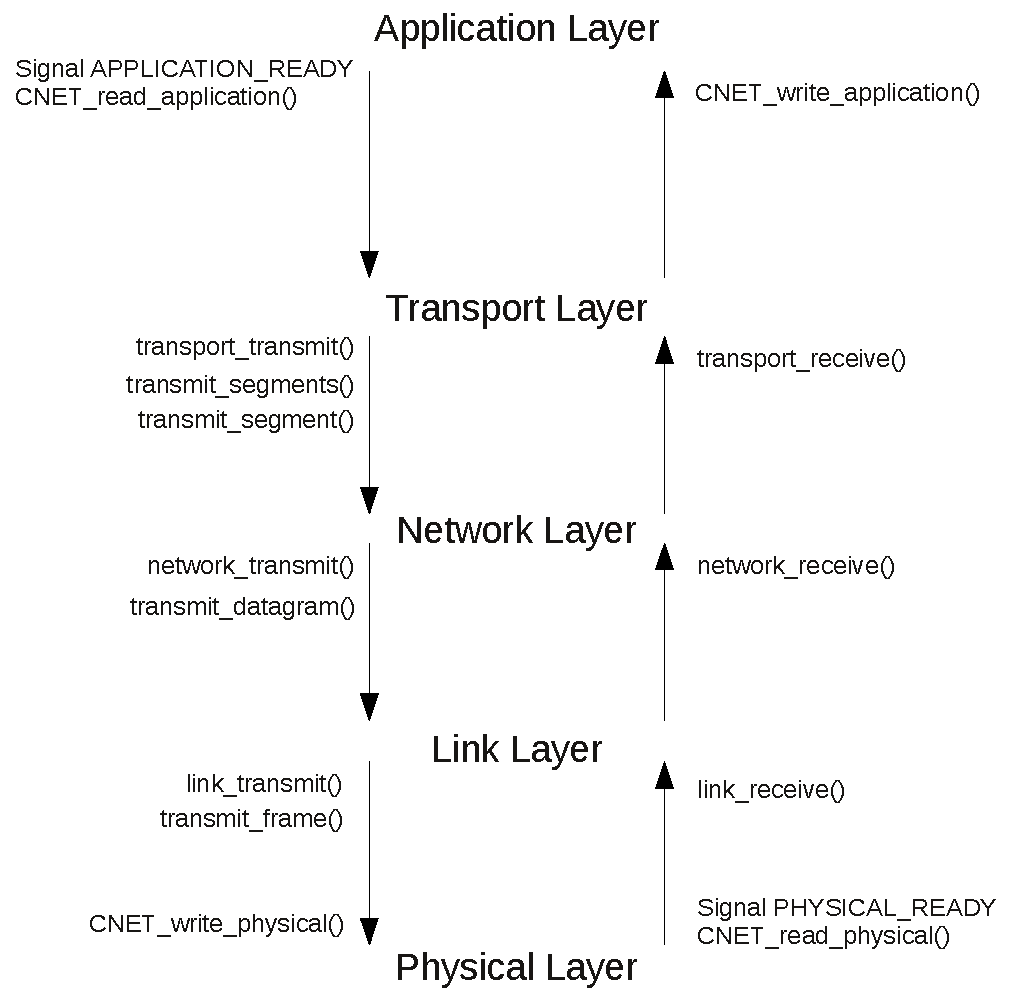
\includegraphics[width=0.9\textwidth]{images/flowgraph_overview.pdf}
  \caption[Overview Layers]{\hcaption{Overview Layers.} Overview of the call hierarchy of the different layers.}
  \label{fig:overview-layers}
\end{figure}


\subsection{Link Layer}
  The link layer provides basic "point2point" connections between neighboring nodes. 

  \subsubsection{Framementation}
  It can handle the transmission of arbitrary large packets (limited by the buffer size, which is large enough to handle all messages in this scenario) independently of the MTU of the link because it has the ability of fra(g)mentation. This means that data from the upper layer is split into several frames, which fit to the MTU minus the additional header information, and put together on the receiver side. Figure~\ref{fig:receiver-side-link-layer} illustrates the receiver side of the link layer. The ordering of the frames is checked by sequence numbers and identification numbers (ID). We use an additional \emph{isLast} flag to identify when a datagram ends. This mechanism is guarded by the fact that no reordering of frames on one link occur. 

  \subsubsection{Corruption Detection}
  This layer also guarantees that all datagrams which are handed to the upper layer are \emph{free of corruption}. Corrupt frames are recognized by computing a checksum and all frames with errors are dropped. \ifthenelse{\boolean{m2}}{We will inspect if it is efficient to implement error correction in this layer.}{We dropped the idea of implementing error correction due to the low rate of corruption.} Finally, the data in this layer are handed to the physical layer in a first come first serve fairness. 

\begin{figure}
  \centering
  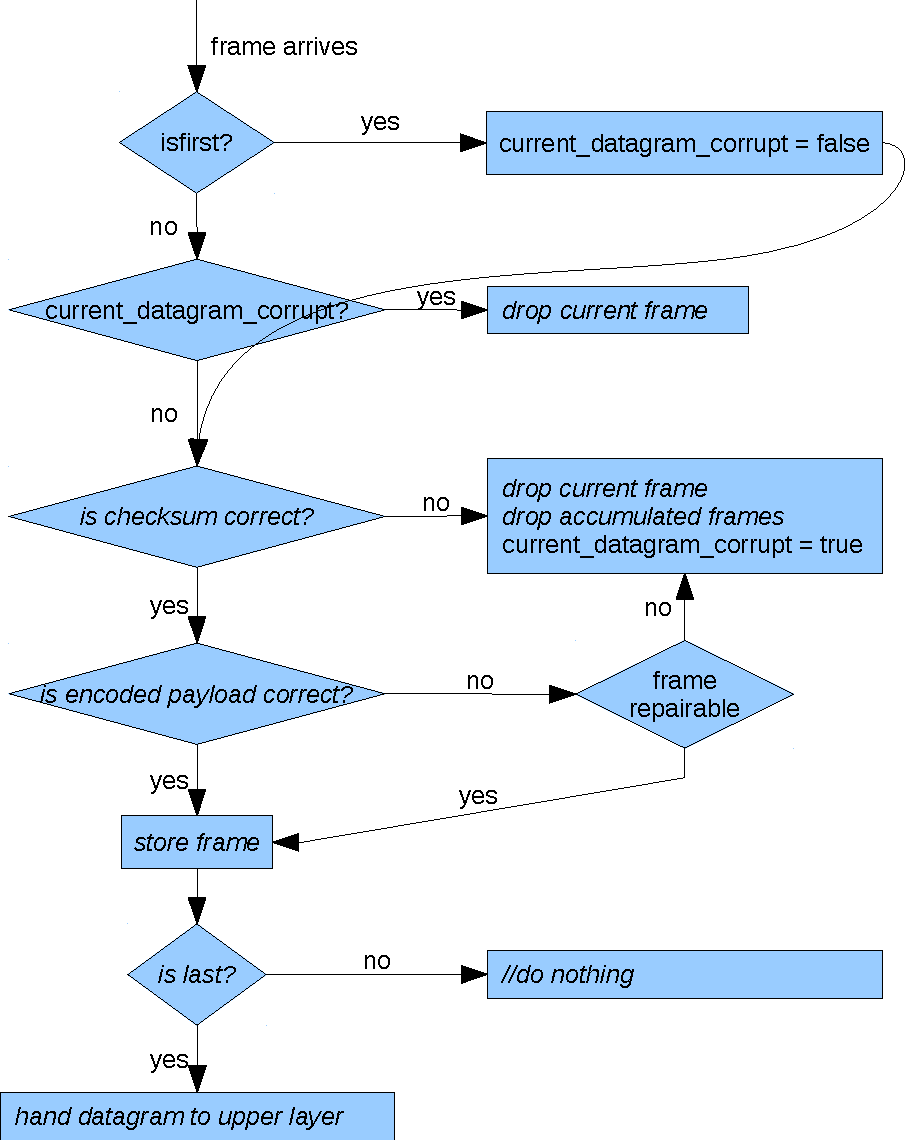
\includegraphics[width=0.9\textwidth]{images/flowgraph_link_layer_receiver.pdf}
  \caption[Receiver side of link layer]{\hcaption{Receiver side of link layer.} The flow graph shows how data on the receiver side of the link layer are handled.}
  \label{fig:receiver-side-link-layer}
\end{figure}

\subsection{Network Layer}

  The network layer has two main tasks: build and maintain a routing / forwarding table as well as route datagrams through the network. 

  \subsubsection{Routing}
  The building and maintaining of the routing table is done in a distributed fashion using the \emph{distance vector algorithm}. Initially, the only information each node has, is, that it can reach itself with cost zero, all other costs are infinity. This corresponds to have routing information for all paths of length zero. Starting from that initial knowledge we will iteratively gain routing information for paths with increasing lengths.

  Whenever a node $i$ receives the routing information that one of his neighbors $j$ can route to an specific destination host $z$ over a path of length $n$ with costs $c$, it concludes that itself could reach that host $z$ over a path of length $n+1$ with costs $c+c(i,j)$ using $j$ as the first hop. Note that $c(i,j)$ is $i$'s cost to reach $j$. The routing table contains information about the costs to reach any node using any of the direct neighbors as next hop. If a routing table update results in a change of the path with the lowest costs, a node broadcasts its new cost to route over that path to all direct neighbors. Thus the routes with minimal costs are propagated through the network.

  As cost or weight function $c(i,j)$ we use the reciprocal of the link bandwidth between node $i$ and node $j$. \fixme{and some more infos, lets see what will be our final decision.}

  Note, that routing information are send in a reliable fashion (using acknowledgments). This ensures that the algorithm terminates with low cost routes for every node.

  Furthermore, a forwarding table is build from the routing table by choosing the neighbor with the minimal costs as the next hop to decrease run time. The forwarding table is kept up to date during the run of the routing algorithm.

  \subsubsection{Forwarding}
  If a datagram arrives at a node, the network layer checks whether this node is indeed the final destination of the datagram. If so the datagram header gets removed and the payload is handed to the transport layer. Otherwise, the datagram is forwarded to the next hop of the path with the minimal costs, according to the forwarding table. On each hop a datagram passes, the hop counter is decreased to avoid that a datagram travels too long in the network.





\subsection{Transport Layer}
  The main task of the transport layer is to provide reliable data transfer and congestion control.

  \subsubsection{Reliable Data Transfer}
  Reliable data transfer means that all messages send on the network will be correctly delivered in order to the application layer of the receiver. To provide this service, the transport layer uses cumulative acknowledgements, sequence numbers in form of offsets and an isLast flag to identify the end of a message. The transport layer has the notion of a connection for all communication partners, i.e. in Cnet that means all other nodes in the system.
  
  In and out going data is buffered per connection. A window is used to send multiple messages without waiting for each acknowledgement, like a stop-and-wait protocol would do. To increase performance we use cumulative acknowledgements where the acknowledgement number is the next offset the connection is waiting for. To provide this in an efficient way, we buffer a limited amount of reordered segments.
  
  Increasing the sequence numbers without a limit is not possible because headers would become larger in size or we would get integer overflows. To control the sequence numbers we use cyclic sequence numbers and also cyclic buffers. The only constraint is that we need more than twice as many sequence numbers as the window is large, to detect the correct order of the sequence numbers.
  
  The calculation of the timeouts is based on the round-trip time (RTT). This is estimated on the basis of exponential weighted moving average of sample RTTs with the suggested values and computation of RFC 2988.
  
  \subsubsection{Congestion Control}
  Additionally this layer provides congestion control using the Reno algorithm explained in the lecture using a slow start and congestion avoidance phase with additive increase and multiplicative decrease as well as the fast recovery phase for three duplicated ACKs.
  
  \subsubsection{Segmentation}
  Due to smaller MTU than the size of the messages we additionally segment messages on this layer to decrease the number of resend messages in case of corruption. If a frame on the link layer gets corrupt, we need to resend the whole segment the whole path the frames have reached previously without errors. If the segments are smaller, the traffic becomes lower.


\section{Results}
\ifthenelse{\boolean{m2}}{% text for milestone 2
  Our analysis shows that throughput and latency stays constant after a short period of time and the number of send / received messages increases linearly as assumed. Figure~\ref{fig:analysis} shows the behavior of the \code{saarnet2.txt} network for a simulation period of 10 min. The fluctuations at the beginning are due to the not filled queues after initialization. With our implementation we reach a throughput from Homburg to Saarbrücken of 9.1 kB/s and 116.8 kB/s the other way around.
  
  \begin{figure}[h]
   \centering
   \subfigure[Throughput]{
    \label{fig:peptide1}
    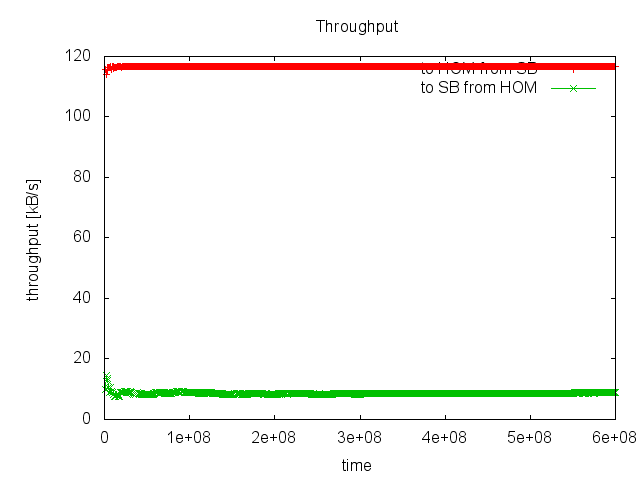
\includegraphics[width=0.48\textwidth]{images/milestone2/results-throughput.png}
   }
   \subfigure[Latency]{
    \label{fig:peptide2}
    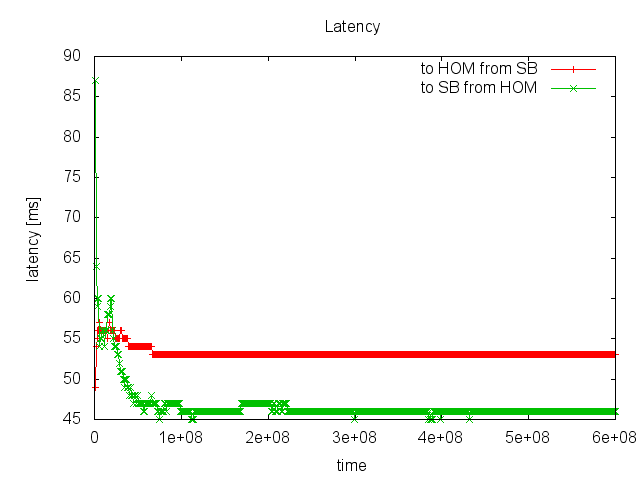
\includegraphics[width=0.48\textwidth]{images/milestone2/results-latency.png}
   }
   \subfigure[Messages]{
    \label{fig:peptide3}
    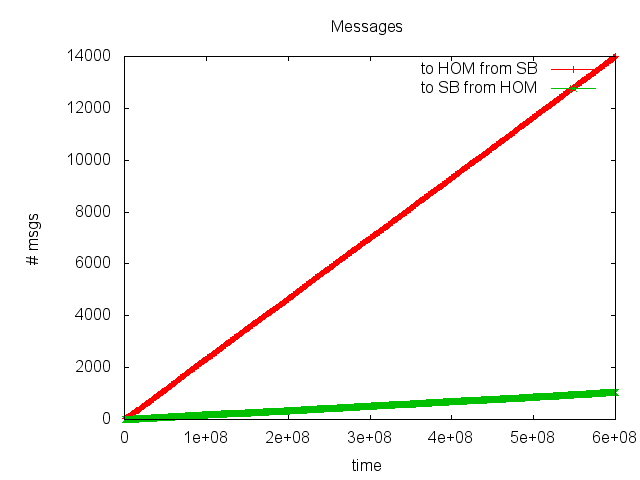
\includegraphics[width=0.48\textwidth]{images/milestone2/results-messages.png}
   }

   \caption[Analysis of milestone 2]{\hcaption{Analysis of milestone 2.} The plots show the behavior for a 10 min simulation of \code{saarnet2.txt}.}
   
   \label{fig:analysis}
  \end{figure}

}{% text for milestone 3
  \fixme{Analysis of milestone 3.}
}

\end{document}
